% =====================================================================
%  Capítulo 17. Modelos con cambios de régimen de Markov
% =====================================================================
\chapter[Cambios de régimen de Markov]{Modelos con cambios de régimen de Markov}\label{cap:markov}

\section*{Objetivos de aprendizaje}
Al terminar este capítulo, el lector podrá:
\begin{enumerate}[label=\arabic*.,leftmargin=*]
  \item Describir una cadena de Markov de dos estados: probabilidades estacionarias, duraciones esperadas y
        persistencia, y demostrar por qué una mezcla con regímenes persistentes produce colas pesadas y
        agrupamiento de volatilidad.
  \item Derivar el filtro de Hamilton, la verosimilitud que produce y el suavizador de Kim.
  \item Estimar los modelos con el algoritmo EM y obtener errores estándar con el hessiano numérico.
  \item Elegir el número de regímenes, interpretarlos frente a cronologías externas como la del NBER y usar el
        modelo para pronosticar y medir el riesgo.
\end{enumerate}

\section*{Motivación}
Los mercados alternan períodos largos de calma con episodios breves de pánico: 1929--1933, 1974, 1987, 2008. Los
modelos GARCH del Capítulo~\ref{cap:garch} describen esa alternancia con una varianza que cambia de forma continua.
Hamilton (1989) propuso otra idea: la economía está en uno de unos pocos \emph{regímenes} (expansión y recesión,
calma y crisis), cada uno con sus propios parámetros, y salta de uno a otro según una cadena de Markov que no se
observa. El econometrista nunca sabe con certeza en qué régimen está, pero puede calcular su probabilidad con los
datos. Ese cálculo, el filtro de Hamilton, es una aplicación directa del teorema de Bayes y la base de este capítulo.

\paragraph{Datos del capítulo.} El exceso de rendimiento mensual del mercado de acciones de EE.\,UU. (factor Mkt-RF de
Kenneth French), de julio de 1926 a noviembre de 2018 ($T=1\,109$); la variación porcentual trimestral del índice de
producción industrial de EE.\,UU. (FRED), de 1970T1 a 2019T2 ($T=198$); y la cronología de picos y valles del ciclo
económico del NBER.

% ---------------------------------------------------------------------
\section{La cadena de Markov}
% ---------------------------------------------------------------------

Sea $s_t\in\{1,\dots,K\}$ el régimen en el período $t$. La cadena es de Markov si el régimen de mañana depende solo
del de hoy:
\[
  \Pr(s_t=j\mid s_{t-1}=i,s_{t-2},\dots)=\Pr(s_t=j\mid s_{t-1}=i)=p_{ij}.
\]
Las probabilidades de transición forman la matriz $P=[p_{ij}]$, cuyas filas suman uno. Con dos regímenes,
\[
  P=\begin{bmatrix}p_{11} & 1-p_{11}\\ 1-p_{22} & p_{22}\end{bmatrix}.
\]

\begin{proposicion}[Propiedades de la cadena de dos estados]\label{prop:cadena}
Si $0<p_{11},p_{22}<1$:
\begin{enumerate}[label=(\alph*)]
  \item La probabilidad estacionaria del régimen 1 es $\pi_1=\dfrac{1-p_{22}}{2-p_{11}-p_{22}}$.
  \item La duración de una estancia en el régimen $i$ es geométrica, con media $\E[D_i]=\dfrac{1}{1-p_{ii}}$.
  \item El indicador $\xi_t=\mathbb 1\{s_t=1\}$ sigue un AR(1): $\E[\xi_{t+1}\mid s_t]=(1-p_{22})+\lambda\,\xi_t$, con
        $\lambda=p_{11}+p_{22}-1$, y su autocorrelación de orden $k$ es $\lambda^k$.
\end{enumerate}
\end{proposicion}

\begin{proof}
(a) La distribución estacionaria cumple $\pi_1=\pi_1p_{11}+\pi_2(1-p_{22})$ y $\pi_2=1-\pi_1$:
\begin{align*}
  \pi_1 &= \pi_1p_{11}+(1-\pi_1)(1-p_{22})\\
  \pi_1 &= \pi_1p_{11}+1-p_{22}-\pi_1+\pi_1p_{22}\\
  \pi_1(2-p_{11}-p_{22}) &= 1-p_{22}\\
  \pi_1 &= \frac{1-p_{22}}{2-p_{11}-p_{22}}.
\end{align*}

(b) Una estancia dura exactamente $d$ períodos si la cadena permanece $d-1$ veces y luego sale:
$\Pr(D_i=d)=p_{ii}^{d-1}(1-p_{ii})$. Usando $\sum_{d\ge1}d\,x^{d-1}=1/(1-x)^2$:
\begin{align*}
  \E[D_i] &= \sum_{d=1}^{\infty}d\,p_{ii}^{d-1}(1-p_{ii})\\
          &= (1-p_{ii})\,\frac{1}{(1-p_{ii})^2}\\
          &= \frac{1}{1-p_{ii}}.
\end{align*}

(c) Si $s_t=1$, $\E[\xi_{t+1}]=p_{11}$; si $s_t=2$, $\E[\xi_{t+1}]=1-p_{22}$. Ambos casos en una fórmula:
\begin{align*}
  \E[\xi_{t+1}\mid s_t] &= p_{11}\,\xi_t+(1-p_{22})(1-\xi_t)\\
                        &= (1-p_{22})+(p_{11}+p_{22}-1)\,\xi_t\\
                        &= (1-p_{22})+\lambda\,\xi_t .
\end{align*}
Es la esperanza condicional de un AR(1) con coeficiente $\lambda$; iterando $k$ veces,
$\E[\xi_{t+k}-\pi_1\mid s_t]=\lambda^k(\xi_t-\pi_1)$, de donde $\operatorname{Corr}(\xi_{t+k},\xi_t)=\lambda^k$.
\end{proof}

Con $p_{11}=0{,}98$ y $p_{22}=0{,}90$, el régimen 1 dura en promedio 50 meses, el 2 dura 10 y la cadena pasa el 83\,\%
del tiempo en el régimen 1. Con $\lambda=0{,}88$ los regímenes son muy persistentes.

% ---------------------------------------------------------------------
\section{El modelo de mezcla con regímenes de Markov}
% ---------------------------------------------------------------------

El modelo más simple con cambio de régimen es
\[
  y_t=\mu_{s_t}+\sigma_{s_t}\varepsilon_t,\qquad \varepsilon_t\sim\text{i.i.d. }N(0,1),
\]
con $\varepsilon_t$ independiente de la cadena. Condicionada en el régimen, $y_t$ es normal; sin conocerlo, es una
\emph{mezcla} de normales con pesos $\pi_j$.

\begin{proposicion}[Momentos de la mezcla]\label{prop:mezcla}
En el estado estacionario, con $\bar\mu=\sum_j\pi_j\mu_j$:
\begin{enumerate}[label=(\alph*)]
  \item $\E[y_t]=\bar\mu$ y $\Var(y_t)=\sum_j\pi_j\sigma_j^2+\sum_j\pi_j(\mu_j-\bar\mu)^2$.
  \item Si $\mu_1=\mu_2$ y $\sigma_1\neq\sigma_2$, la curtosis es mayor que 3.
  \item Si $\mu_1=\mu_2=0$, $\Cov(y_t^2,y_{t-k}^2)=(\sigma_1^2-\sigma_2^2)^2\,\pi_1\pi_2\,\lambda^k$.
\end{enumerate}
\end{proposicion}

\begin{proof}
(a) Por la ley de la varianza total, condicionando en el régimen:
\begin{align*}
  \Var(y_t) &= \E\bigl[\Var(y_t\mid s_t)\bigr]+\Var\bigl(\E[y_t\mid s_t]\bigr)\\
            &= \sum_j\pi_j\sigma_j^2+\sum_j\pi_j(\mu_j-\bar\mu)^2 .
\end{align*}

(b) Con media común $\mu$, sean $m_2=\sum_j\pi_j\sigma_j^2$ y $m_4=\E[(y_t-\mu)^4]$. Como el cuarto momento de una normal es
$3\sigma^4$:
\begin{align*}
  m_4 &= \sum_j\pi_j\,3\sigma_j^4\\
      &= 3\,\E[\sigma_{s_t}^4]\\
      &> 3\,\bigl(\E[\sigma_{s_t}^2]\bigr)^2\\
      &= 3\,m_2^2,
\end{align*}
donde la desigualdad es la de Jensen ($\Var(\sigma^2_{s_t})>0$ porque las varianzas difieren). La curtosis es
$m_4/m_2^2>3$.

(c) Con $\mu_j=0$, $\E[y_t^2\mid s_t]=\sigma_{s_t}^2=\sigma_2^2+(\sigma_1^2-\sigma_2^2)\,\xi_t$. Como los $\varepsilon$ son independientes
de la cadena y entre sí, para $k\ge1$:
\begin{align*}
  \Cov(y_t^2,y_{t-k}^2) &= \Cov\bigl(\E[y_t^2\mid s],\ \E[y_{t-k}^2\mid s]\bigr)\\
                        &= \Cov\bigl(\sigma_2^2+(\sigma_1^2-\sigma_2^2)\xi_t,\ \sigma_2^2+(\sigma_1^2-\sigma_2^2)\xi_{t-k}\bigr)\\
                        &= (\sigma_1^2-\sigma_2^2)^2\,\Cov(\xi_t,\xi_{t-k})\\
                        &= (\sigma_1^2-\sigma_2^2)^2\,\pi_1\pi_2\,\lambda^k,
\end{align*}
usando $\Var(\xi_t)=\pi_1\pi_2$ y la parte (c) de la Proposición~\ref{prop:cadena}.
\end{proof}

La proposición explica por qué estos modelos encajan con los hechos estilizados del Capítulo~\ref{cap:hechos}: la mezcla
genera colas pesadas, y la persistencia de los regímenes genera autocorrelación positiva y lenta de los cuadrados, es
decir, agrupamiento de volatilidad. La Figura~\ref{fig:regimenes} lo muestra con $\mu=(1;\,-0{,}5)$, $\sigma=(3{,}5;\,8)$,
$p_{11}=0{,}98$ y $p_{22}=0{,}90$: la mezcla tiene curtosis 5,63, frente a 3 de la normal con la misma media y varianza.

\begin{figure}[ht]
\centering
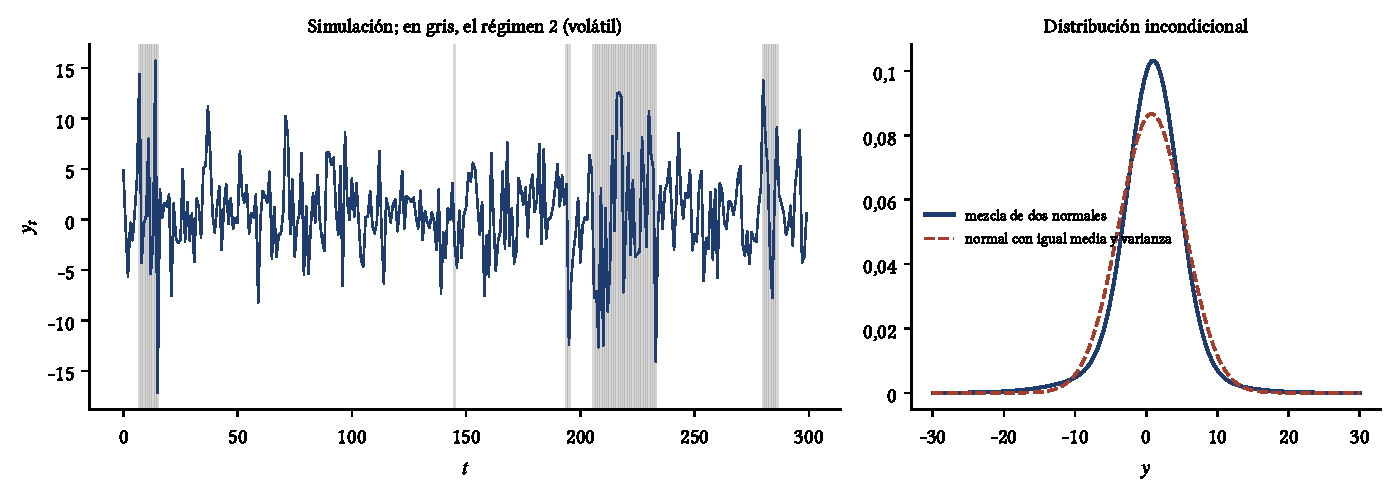
\includegraphics[width=\linewidth]{graficos/cap17_fig_regimenes.pdf}
\caption{Izquierda: 300 observaciones simuladas de un modelo con dos regímenes; en gris, los períodos en el régimen
volátil. Derecha: la distribución incondicional (mezcla) frente a la normal de igual media y varianza: más alta en el
centro y con colas más gruesas.}
\label{fig:regimenes}
\end{figure}

% ---------------------------------------------------------------------
\section{El filtro de Hamilton}
% ---------------------------------------------------------------------

Sean $\mathcal Y_t=(y_1,\dots,y_t)$ la información hasta $t$, $\eta_{jt}=f(y_t\mid s_t=j,\mathcal Y_{t-1})$ la densidad en el
régimen $j$ (en el modelo de mezcla, $\phi\bigl((y_t-\mu_j)/\sigma_j\bigr)/\sigma_j$) y los vectores de probabilidades
\[
  \boldsymbol\xi_{t\mid t-1}=\bigl[\Pr(s_t=j\mid\mathcal Y_{t-1})\bigr]_j\ \ \text{(predichas)},\qquad
  \boldsymbol\xi_{t\mid t}=\bigl[\Pr(s_t=j\mid\mathcal Y_t)\bigr]_j\ \ \text{(filtradas)}.
\]

\begin{proposicion}[Filtro de Hamilton]\label{prop:hamilton}
Partiendo de $\boldsymbol\xi_{1\mid0}=\boldsymbol\rho$, para $t=1,\dots,T$:
\[
  f(y_t\mid\mathcal Y_{t-1})=\sum_j\xi_{j,t\mid t-1}\,\eta_{jt},\qquad
  \xi_{j,t\mid t}=\frac{\xi_{j,t\mid t-1}\,\eta_{jt}}{f(y_t\mid\mathcal Y_{t-1})},\qquad
  \boldsymbol\xi_{t+1\mid t}=P'\boldsymbol\xi_{t\mid t},
\]
y la log-verosimilitud es $\ell=\sum_{t=1}^T\ln f(y_t\mid\mathcal Y_{t-1})$.
\end{proposicion}

\begin{proof}
La densidad de $y_t$ dada la historia se obtiene sumando sobre el régimen (ley de probabilidad total):
\begin{align*}
  f(y_t\mid\mathcal Y_{t-1}) &= \sum_j f(y_t,s_t=j\mid\mathcal Y_{t-1})\\
                             &= \sum_j\Pr(s_t=j\mid\mathcal Y_{t-1})\,f(y_t\mid s_t=j,\mathcal Y_{t-1})\\
                             &= \sum_j\xi_{j,t\mid t-1}\,\eta_{jt}.
\end{align*}
La actualización es el teorema de Bayes:
\begin{align*}
  \Pr(s_t=j\mid\mathcal Y_t) &= \frac{f(y_t,s_t=j\mid\mathcal Y_{t-1})}{f(y_t\mid\mathcal Y_{t-1})}\\
                             &= \frac{\xi_{j,t\mid t-1}\,\eta_{jt}}{f(y_t\mid\mathcal Y_{t-1})}.
\end{align*}
La predicción usa la propiedad de Markov, $\Pr(s_{t+1}=j\mid s_t=i,\mathcal Y_t)=p_{ij}$:
\begin{align*}
  \Pr(s_{t+1}=j\mid\mathcal Y_t) &= \sum_i\Pr(s_t=i\mid\mathcal Y_t)\,p_{ij}\\
                                 &= \bigl[P'\boldsymbol\xi_{t\mid t}\bigr]_j .
\end{align*}
Finalmente, la densidad conjunta se factoriza en condicionales:
\begin{align*}
  \ln f(y_1,\dots,y_T) &= \ln\prod_{t=1}^Tf(y_t\mid\mathcal Y_{t-1})\\
                       &= \sum_{t=1}^T\ln f(y_t\mid\mathcal Y_{t-1}).
\end{align*}
\end{proof}

\begin{proposicion}[Suavizador de Kim]\label{prop:kim}
Con $\boldsymbol\xi_{T\mid T}$ del filtro, hacia atrás para $t=T-1,\dots,1$:
\[
  \xi_{i,t\mid T}=\xi_{i,t\mid t}\sum_j p_{ij}\,\frac{\xi_{j,t+1\mid T}}{\xi_{j,t+1\mid t}},\qquad
  \Pr(s_t=i,s_{t+1}=j\mid\mathcal Y_T)=\frac{\xi_{i,t\mid t}\,p_{ij}\,\xi_{j,t+1\mid T}}{\xi_{j,t+1\mid t}}.
\]
\end{proposicion}

\begin{proof}
El paso clave es que, conocido $s_{t+1}$, las observaciones futuras no informan sobre $s_t$:
$\Pr(s_t=i\mid s_{t+1}=j,\mathcal Y_T)=\Pr(s_t=i\mid s_{t+1}=j,\mathcal Y_t)$, porque $y_{t+1},\dots,y_T$ dependen de $s_t$ solo
a través de $s_{t+1}$ (supuesto exacto en el modelo de mezcla y en el MSI-AR del Ejercicio~\ref{ej:produccion}). Por Bayes:
\begin{align*}
  \Pr(s_t=i\mid s_{t+1}=j,\mathcal Y_t) &= \frac{\Pr(s_t=i\mid\mathcal Y_t)\,\Pr(s_{t+1}=j\mid s_t=i)}{\Pr(s_{t+1}=j\mid\mathcal Y_t)}\\
                                         &= \frac{\xi_{i,t\mid t}\,p_{ij}}{\xi_{j,t+1\mid t}}.
\end{align*}
Multiplicando por $\Pr(s_{t+1}=j\mid\mathcal Y_T)$ se obtiene la probabilidad conjunta, y sumando sobre $j$, la marginal:
\begin{align*}
  \Pr(s_t=i,s_{t+1}=j\mid\mathcal Y_T) &= \frac{\xi_{i,t\mid t}\,p_{ij}\,\xi_{j,t+1\mid T}}{\xi_{j,t+1\mid t}},\\
  \xi_{i,t\mid T} &= \sum_j\frac{\xi_{i,t\mid t}\,p_{ij}\,\xi_{j,t+1\mid T}}{\xi_{j,t+1\mid t}}\\
                  &= \xi_{i,t\mid t}\sum_jp_{ij}\,\frac{\xi_{j,t+1\mid T}}{\xi_{j,t+1\mid t}}.
\end{align*}
\end{proof}

Las probabilidades \emph{filtradas} usan solo el pasado y son las que habría calculado un inversionista en tiempo
real; las \emph{suavizadas} usan toda la muestra y son las adecuadas para fechar los regímenes después.

% ---------------------------------------------------------------------
\section{Estimación por el algoritmo EM}
% ---------------------------------------------------------------------

La verosimilitud de la Proposición~\ref{prop:hamilton} puede maximizarse numéricamente, pero tiene muchos óptimos
locales y restricciones ($0<p_{ij}<1$, $\sigma_j>0$). El algoritmo EM (Dempster, Laird y Rubin, 1977; Hamilton, 1990)
es más estable: si los regímenes se observaran, estimar el modelo sería trivial; como no se observan, se sustituyen
por sus probabilidades suavizadas y se itera.

\begin{proposicion}[Paso M del modelo de mezcla]\label{prop:em}
Dadas las probabilidades suavizadas $\hat\xi_{jt}=\Pr(s_t=j\mid\mathcal Y_T)$ y
$\hat n_{ij}=\sum_{t=2}^T\Pr(s_{t-1}=i,s_t=j\mid\mathcal Y_T)$ calculadas con los parámetros actuales, los valores que
maximizan la log-verosimilitud completa esperada son
\[
  \hat\mu_j=\frac{\sum_t\hat\xi_{jt}\,y_t}{\sum_t\hat\xi_{jt}},\qquad
  \hat\sigma_j^2=\frac{\sum_t\hat\xi_{jt}\,(y_t-\hat\mu_j)^2}{\sum_t\hat\xi_{jt}},\qquad
  \hat p_{ij}=\frac{\hat n_{ij}}{\sum_k\hat n_{ik}} .
\]
\end{proposicion}

\begin{proof}
Si los regímenes se observaran, la log-verosimilitud completa sería
$\sum_t\sum_j\mathbb 1\{s_t=j\}\ln\eta_{jt}+\sum_t\sum_{i,j}\mathbb 1\{s_{t-1}=i,s_t=j\}\ln p_{ij}$, más un término de la
probabilidad inicial. Su esperanza condicional en los datos sustituye los indicadores por las probabilidades suavizadas:
\[
  Q=\sum_t\sum_j\hat\xi_{jt}\Bigl[-\tfrac12\ln(2\pi\sigma_j^2)-\frac{(y_t-\mu_j)^2}{2\sigma_j^2}\Bigr]+\sum_{i,j}\hat n_{ij}\ln p_{ij}.
\]
Para $\mu_j$:
\begin{align*}
  \frac{\partial Q}{\partial\mu_j} &= \sum_t\hat\xi_{jt}\,\frac{y_t-\mu_j}{\sigma_j^2}=0\\
  \sum_t\hat\xi_{jt}\,y_t &= \mu_j\sum_t\hat\xi_{jt}\\
  \hat\mu_j &= \frac{\sum_t\hat\xi_{jt}\,y_t}{\sum_t\hat\xi_{jt}}.
\end{align*}
Para $\sigma_j^2$:
\begin{align*}
  \frac{\partial Q}{\partial\sigma_j^2} &= \sum_t\hat\xi_{jt}\Bigl[-\frac{1}{2\sigma_j^2}+\frac{(y_t-\mu_j)^2}{2\sigma_j^4}\Bigr]=0\\
  \sigma_j^2\sum_t\hat\xi_{jt} &= \sum_t\hat\xi_{jt}(y_t-\mu_j)^2 .
\end{align*}
Para cada fila $i$ de $P$ maximizamos $\sum_j\hat n_{ij}\ln p_{ij}$ sujeto a $\sum_jp_{ij}=1$, con el lagrangiano
$\sum_j\hat n_{ij}\ln p_{ij}-\kappa(\sum_jp_{ij}-1)$:
\begin{align*}
  \frac{\hat n_{ij}}{p_{ij}}-\kappa &= 0\\
  p_{ij} &= \hat n_{ij}/\kappa\\
  \sum_jp_{ij}=1 &\ \Rightarrow\ \kappa=\sum_k\hat n_{ik}\\
  \hat p_{ij} &= \frac{\hat n_{ij}}{\sum_k\hat n_{ik}} .
\end{align*}
\end{proof}

El paso M es una media y una varianza \emph{ponderadas} por la probabilidad de cada régimen, y la transición estimada es
la frecuencia esperada de pasar de $i$ a $j$. Cada iteración EM no disminuye la verosimilitud; se itera hasta que el
aumento sea menor que $10^{-10}$. En el modelo MSI-AR del Ejercicio~\ref{ej:produccion}, con intercepto cambiante y
$\phi$ y $\sigma$ comunes, el paso M es una regresión de mínimos cuadrados ponderados con una ficticia por régimen.

\begin{observacion}[Identificación y número de regímenes]
Los regímenes solo están definidos salvo una permutación: cambiar los nombres de 1 y 2 da la misma verosimilitud. Se
fija el orden con una regla, por ejemplo $\sigma_1<\sigma_2$. Contrastar $K=1$ frente a $K=2$ con la razón de
verosimilitudes no es estándar: bajo la hipótesis nula, $p_{11}$ y $p_{22}$ no están identificados y el estadístico no
sigue una $\chi^2$ (Hansen, 1992; Garcia, 1998). En la práctica se usan criterios de información, el bootstrap
paramétrico o, como en el Ejercicio~\ref{ej:numero}, contrastes \emph{dentro} de un modelo con el mismo número de regímenes,
que sí son estándar.
\end{observacion}

% ---------------------------------------------------------------------
\section{Ejercicios resueltos}
% ---------------------------------------------------------------------

\begin{ejresuelto}{Dos regímenes en el mercado de EE.\,UU.}\label{ej:mercado2}
\enunciado Estime por EM el modelo $y_t=\mu_{s_t}+\sigma_{s_t}\varepsilon_t$ con dos regímenes para el exceso de rendimiento
mensual del mercado de 1926 a 2018. Calcule errores estándar con el hessiano numérico, las probabilidades estacionarias, las
duraciones y los momentos implícitos, y compare con la normal.

\solucion
\paso{Paso 1. Estimaciones.} El EM converge en 53 iteraciones a $\ell=-3\,256{,}22$:
\begin{center}\small
\begin{tabular}{@{}lrrlrr@{}}
\toprule
 & Régimen 1 (tranquilo) & ee & & Régimen 2 (volátil) & ee \\
\midrule
$\mu_j$ (\%) & 1,009 & 0,143 & & $-1{,}430$ & 0,880 \\
$\sigma_j$ (\%) & 3,741 & 0,133 & & 10,456 & 0,864 \\
$p_{jj}$ & 0,9842 & 0,007 & & 0,9058 & 0,037 \\
\bottomrule
\end{tabular}
\end{center}
En el régimen tranquilo el mercado rinde un 1,01\,\% mensual sobre la tasa libre de riesgo con una volatilidad de 3,7\,\%;
en el volátil, la volatilidad casi se triplica y el rendimiento medio es negativo, aunque impreciso.

\paso{Paso 2. Persistencia.} Por la Proposición~\ref{prop:cadena}:
\begin{align*}
  \E[D_1] &= \frac{1}{1-0{,}9842}\\
          &= 63{,}3\ \text{meses},\\
  \E[D_2] &= \frac{1}{1-0{,}9058}\\
          &= 10{,}6\ \text{meses},\\
  \pi_1 &= \frac{1-0{,}9058}{2-0{,}9842-0{,}9058}\\
        &= \frac{0{,}0942}{0{,}1100}\\
        &= 0{,}856 .
\end{align*}
El mercado pasa el 86\,\% del tiempo en calma, en episodios de más de cinco años, y el 14\,\% en crisis que duran en promedio
casi un año ($\lambda=0{,}89$).

\paso{Paso 3. Momentos y ajuste.} El modelo reproduce la media (0,659) y la desviación estándar (5,329) de la muestra, e
implica una curtosis de 7,52 frente a 10,90 en los datos: captura gran parte de las colas pesadas, aunque no todas. La
log-verosimilitud mejora en 172,1 puntos sobre la normal (Figura~\ref{fig:densidad17}). La razón de Sharpe mensual es 0,27
en el régimen tranquilo y $-0{,}14$ en el volátil (Figura~\ref{fig:prob17}).

\codigoweb{cap17_ej01}
\salidaR{cap17_ej01_R.txt}
\lectura{cap17_ej01}

\RvsPy El filtro, el suavizador y el EM están programados igual en ambos lenguajes y producen las mismas cifras. El EM es
determinista: con los mismos valores iniciales y el mismo criterio de parada, R y Python recorren las mismas iteraciones. Los
errores estándar salen de un hessiano numérico por diferencias centrales y difieren en la cuarta decimal por redondeo; por eso
se imprimen con tres. Como verificación, \texttt{statsmodels} (\texttt{MarkovRegression} con \texttt{switching\_variance=True}),
que maximiza la verosimilitud directamente y fija la probabilidad inicial en la estacionaria, da $\ell=-3\,256{,}37$,
$\mu=(1{,}007;\,-1{,}435)$ y $\sigma=(3{,}743;\,10{,}470)$ (archivo \texttt{cap17\_ej01\_statsmodels.py}). La pequeña diferencia en $\ell$ se
debe a que nuestro EM estima también la probabilidad inicial.

\begin{figure}[ht]
\centering
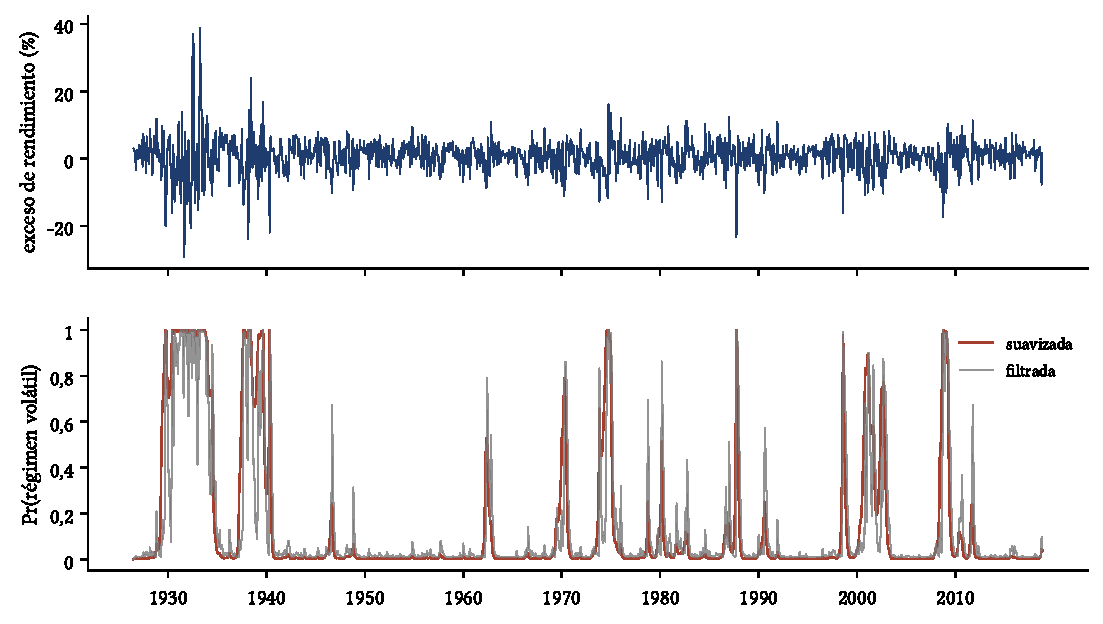
\includegraphics[width=\linewidth]{graficos/cap17_ej01_probabilidades.pdf}
\caption{Arriba: exceso de rendimiento mensual del mercado. Abajo: probabilidad del régimen volátil, filtrada (gris) y
suavizada (rojo). Destacan los episodios de 1929--1934, 1937--1940, 1974, 2000--2002 y 2008--2009.}
\label{fig:prob17}
\end{figure}

\begin{figure}[ht]
\centering
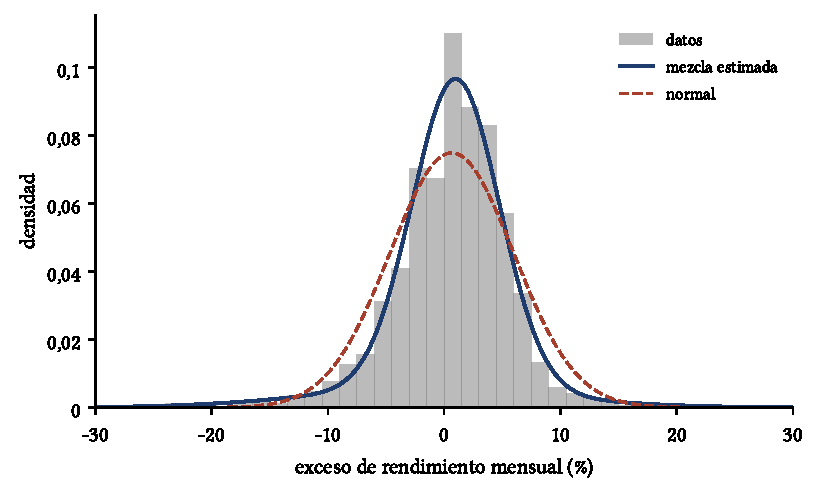
\includegraphics[width=0.75\linewidth]{graficos/cap17_ej01_densidad.pdf}
\caption{Histograma de los rendimientos con la mezcla estimada y la normal de igual media y varianza.}
\label{fig:densidad17}
\end{figure}

\begin{conclusion}
Dos regímenes bastan para describir la mayor parte de las colas pesadas y del agrupamiento de volatilidad del mercado
estadounidense: un régimen largo y tranquilo con prima positiva y otro corto y turbulento con prima negativa.
\end{conclusion}
\end{ejresuelto}

\begin{ejresuelto}{El régimen volátil y las recesiones}\label{ej:nber}
\enunciado Compare la probabilidad suavizada del régimen volátil del Ejercicio~\ref{ej:mercado2} con la cronología de recesiones del
NBER (un mes está en recesión desde el mes siguiente al pico hasta el valle). Identifique los episodios volátiles de seis meses
o más.

\solucion
\paso{Paso 1. Asociación.} Hay 199 meses de recesión en la muestra. La probabilidad media del régimen volátil es 0,437 en
recesión y 0,079 en expansión, y la correlación con el indicador de recesión es 0,466.
\begin{center}\small
\begin{tabular}{@{}lrr@{}}
\toprule
NBER & Tranquilo & Volátil \\
\midrule
Expansión & 852 & 58 \\
Recesión & 110 & 89 \\
\bottomrule
\end{tabular}
\end{center}
\begin{align*}
  \Pr(\text{volátil}\mid\text{recesión}) &= \frac{89}{199}\\
                                       &= 0{,}447,\\
  \Pr(\text{volátil}\mid\text{expansión}) &= \frac{58}{910}\\
                                        &= 0{,}064 .
\end{align*}

\paso{Paso 2. Episodios.}
\begin{center}\small
\begin{tabular}{@{}llrrrr@{}}
\toprule
Inicio & Fin & Meses & Media (\%) & Desv.\ est.\ (\%) & Meses en recesión \\
\midrule
1929-05 & 1934-07 & 63 & $-0{,}71$ & 12,77 & 43 \\
1937-06 & 1939-10 & 29 & 0,13 & 9,69 & 13 \\
1970-01 & 1970-06 & 6 & $-4{,}62$ & 5,28 & 6 \\
1974-03 & 1975-01 & 11 & $-2{,}09$ & 8,46 & 11 \\
2000-09 & 2001-09 & 13 & $-3{,}31$ & 5,36 & 6 \\
2008-08 & 2009-04 & 9 & $-3{,}35$ & 8,82 & 9 \\
\bottomrule
\end{tabular}
\end{center}
La Gran Depresión, la recesión de 1937--1938, la crisis petrolera de 1974, el fin de la burbuja tecnológica y la crisis
financiera de 2008 son regímenes volátiles. Pero muchas recesiones de posguerra (1948, 1953, 1957, 1960, 1981--1982, 1990)
tienen probabilidad casi nula: no todas las recesiones son crisis bursátiles, y no todas las crisis bursátiles son recesiones
(Figura~\ref{fig:nber}).

\codigoweb{cap17_ej02}
\salidaR{cap17_ej02_R.txt}
\lectura{cap17_ej02}

\RvsPy Los episodios consecutivos se encuentran en R con \texttt{rle} (\emph{run-length encoding}), que devuelve la longitud
y el valor de cada racha; en Python, con un bucle que avanza mientras el régimen no cambia. Las fechas en formato
\texttt{AAAA-MM} se comparan como texto: el orden alfabético coincide con el cronológico.

\begin{figure}[ht]
\centering
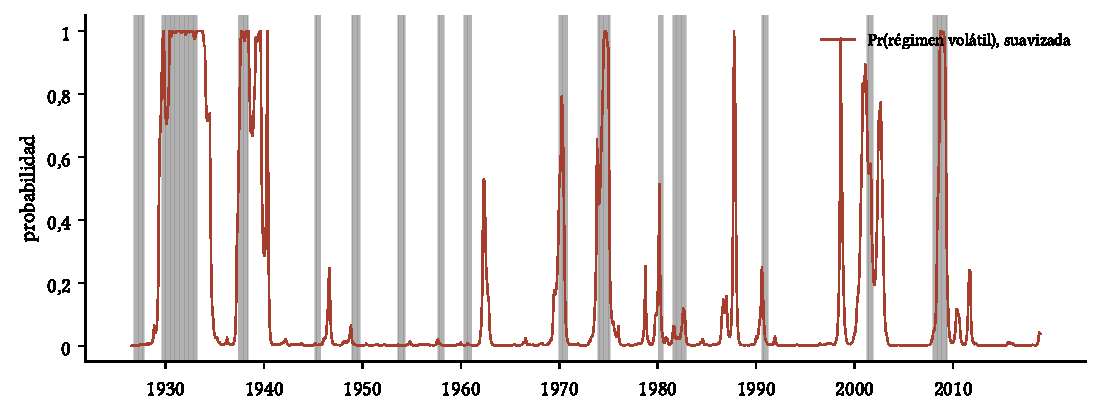
\includegraphics[width=\linewidth]{graficos/cap17_ej02_nber.pdf}
\caption{Probabilidad suavizada del régimen volátil y recesiones del NBER (franjas grises).}
\label{fig:nber}
\end{figure}

\begin{conclusion}
El régimen volátil está asociado con las recesiones, pero no las identifica: lo determinan las crisis financieras más que el
ciclo real. Fechar el ciclo exige un modelo para una variable real, que es el ejercicio siguiente.
\end{conclusion}
\end{ejresuelto}

\begin{ejresuelto}{El ciclo de la producción industrial}\label{ej:produccion}
\enunciado Con la variación trimestral de la producción industrial de 1970 a 2019, estime (A) el modelo MSI-AR(1)
$y_t=c_{s_t}+\phi\,y_{t-1}+\sigma\varepsilon_t$, con varianza común, y (B) el modelo de media y varianza cambiantes. Compare
ambos con los 29 trimestres de recesión del NBER (un trimestre está en recesión si al menos dos de sus meses lo están).

\solucion
\paso{Paso 1. Modelo A.} El AR(1) lineal tiene $\hat\phi=0{,}579$ y $\ell=-319{,}23$. El MSI-AR(1) mejora la verosimilitud a
$\ell=-299{,}37$ con $c_1=-3{,}671$, $c_2=0{,}440$, $\phi=0{,}431$ y $\sigma=0{,}998$. Pero su régimen 1 dura en promedio
\begin{align*}
  \frac{1}{1-0{,}4722} &= 1{,}89\ \text{trimestres}
\end{align*}
y solo clasifica 6 trimestres: los desplomes de 1974--1975, 1980, 1981 y 2008--2009. El modelo usa el segundo régimen para
acomodar los valores extremos, no para describir el ciclo.

\paso{Paso 2. Modelo B.} Con media y varianza cambiantes, $\ell=-319{,}45$:
\begin{center}\small
\begin{tabular}{@{}lrrrr@{}}
\toprule
Régimen & $\mu_j$ & $\sigma_j$ & $p_{jj}$ & Duración (trim.) \\
\midrule
1 (recesión) & $-1{,}452$ & 1,901 & 0,7749 & 4,44 \\
2 (expansión) & 0,984 & 0,907 & 0,9503 & 20,13 \\
\bottomrule
\end{tabular}
\end{center}
Ahora el régimen 1 es una recesión típica: la producción cae 1,45\,\% por trimestre durante algo más de un año. De los 36 trimestres
clasificados en recesión, 25 coinciden con el NBER, hay 11 falsas alarmas (seis de ellas en la contracción industrial de 2015--2016,
que el NBER no consideró recesión) y solo 4 recesiones no detectadas. La concordancia es 0,924 y la correlación con el indicador
NBER, 0,802 (Figura~\ref{fig:produccion}).

\paso{Paso 3. ¿Cuál es mejor?} A tiene mayor verosimilitud, pero B describe el ciclo. Las verosimilitudes no son del todo
comparables (A condiciona en la primera observación), y B ignora la autocorrelación dentro de cada régimen: la
autocorrelación de $y_t$ menos su media suavizada es aún 0,378. El modelo de Hamilton (1989), con intercepto y media cambiantes
en un AR(4), resuelve ambos problemas a costa de un paso M más complejo. La lección general es que la verosimilitud por sí sola
no garantiza que los regímenes tengan la interpretación buscada.

\codigoweb{cap17_ej03}
\salidaR{cap17_ej03_R.txt}
\lectura{cap17_ej03}

\RvsPy El paso M del MSI-AR resuelve un sistema de $K+1$ ecuaciones normales ponderadas, con \texttt{solve} en R y
\texttt{np.linalg.solve} en Python. Probamos 18 combinaciones de valores iniciales con el modelo A y 3 con el B, y en cada modelo todas
convergen al mismo máximo, lo que hace improbable que A sea un óptimo local. El indicador trimestral de recesión se construye a partir del mensual, con
\texttt{sprintf("\%s-\%02d", ...)} en R y una comprensión de listas en Python.

\begin{figure}[ht]
\centering
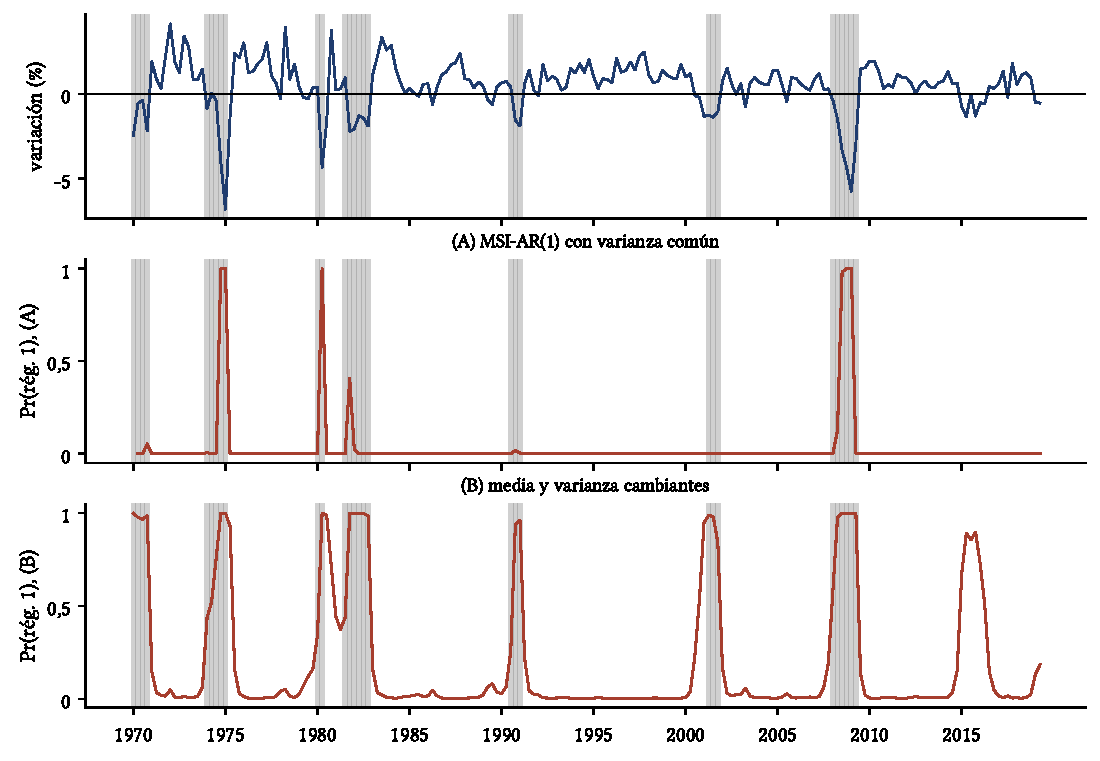
\includegraphics[width=\linewidth]{graficos/cap17_ej03_produccion.pdf}
\caption{Arriba: variación trimestral de la producción industrial. Al medio y abajo: probabilidad suavizada del régimen 1 en
los modelos A y B. Franjas grises: trimestres de recesión del NBER.}
\label{fig:produccion}
\end{figure}

\begin{conclusion}
Con media y varianza cambiantes, un modelo de dos regímenes reproduce la cronología del NBER sin usarla, a partir de una sola
serie. El modelo de mayor verosimilitud, en cambio, dedica un régimen a los valores atípicos.
\end{conclusion}
\end{ejresuelto}

\begin{ejresuelto}{¿Cuántos regímenes?}\label{ej:numero}
\enunciado Para el mercado, compare un régimen (normal), dos regímenes solo en la varianza, dos en media y varianza y tres en
media y varianza, con AIC y BIC. Contraste si las medias de los dos regímenes son iguales.

\solucion
\paso{Paso 1. Criterios de información.}
\begin{center}\small
\begin{tabular}{@{}lrrrr@{}}
\toprule
Modelo & $k$ & $\ell$ & AIC & BIC \\
\midrule
1 régimen (normal) & 2 & $-3\,428{,}33$ & 6\,860,67 & 6\,870,69 \\
2 regímenes, solo varianza & 5 & $-3\,260{,}73$ & 6\,531,45 & 6\,556,51 \\
2 regímenes, media y varianza & 6 & $-3\,256{,}22$ & 6\,524,45 & 6\,554,52 \\
3 regímenes, media y varianza & 12 & $-3\,234{,}26$ & 6\,492,52 & 6\,552,66 \\
\bottomrule
\end{tabular}
\end{center}
El salto de uno a dos regímenes es enorme; el de dos a tres es menor y el BIC apenas lo prefiere (por 1,86 puntos).

\paso{Paso 2. Medias iguales.} Con dos regímenes identificados por la varianza, la hipótesis $\mu_1=\mu_2$ es un contraste
estándar:
\begin{align*}
  LR &= 2\,\bigl[-3\,256{,}2248-(-3\,260{,}7262)\bigr]\\
     &= 2\times4{,}5014\\
     &= 9{,}003,
\end{align*}
con valor $p=0{,}0027$ en una $\chi^2_1$: el rendimiento medio sí cambia con el régimen.

\paso{Paso 3. Tres regímenes.} Aparecen un régimen muy tranquilo ($\sigma=2{,}72$, $\mu=1{,}22$), uno intermedio
($\sigma=4{,}52$, $\mu=0{,}67$) y uno de crisis ($\sigma=11{,}92$, $\mu=-1{,}29$), con duraciones de 24, 28 y 12 meses. La matriz de
transición es casi tridiagonal: de la calma no se salta directamente a la crisis (probabilidad estimada 0,0000), sino que se
pasa por el régimen intermedio (Figura~\ref{fig:tres}).

\codigoweb{cap17_ej04}
\salidaR{cap17_ej04_R.txt}
\lectura{cap17_ej04}

\RvsPy La función \texttt{em\_media\_varianza} sirve para cualquier $K$ y para el caso de media común
(\texttt{media\_comun}). En la tabla de salida el nombre del modelo va al final de cada línea: \texttt{sprintf} de R rellena
el ancho contando bytes, de modo que un nombre con tildes queda desalineado respecto de Python, que cuenta caracteres.

\begin{figure}[ht]
\centering
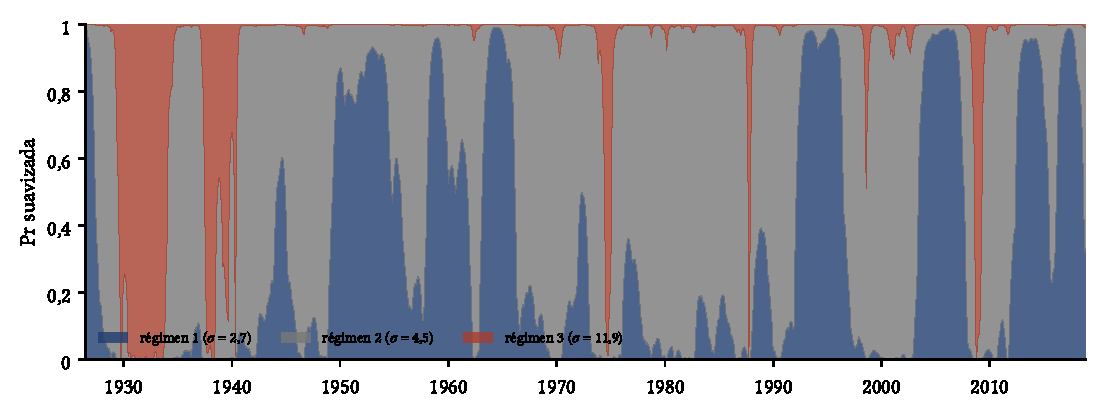
\includegraphics[width=\linewidth]{graficos/cap17_ej04_tres_regimenes.pdf}
\caption{Probabilidades suavizadas del modelo de tres regímenes, apiladas. El régimen de crisis (rojo) se concentra en
1929--1934, 1937--1940, 1974, 1987 y 2008--2009.}
\label{fig:tres}
\end{figure}

\begin{conclusion}
Los datos piden al menos dos regímenes que difieran en media y varianza. Un tercero mejora el ajuste y tiene una lectura
económica razonable, pero la evidencia a su favor es débil y, con 12 parámetros, sus estimaciones son menos estables.
\end{conclusion}
\end{ejresuelto}

\begin{ejresuelto}{Pronóstico y VaR con regímenes}\label{ej:var17}
\enunciado Con el modelo de dos regímenes, pronostique la media, la volatilidad y el VaR del mes siguiente a noviembre de 2018.
Luego evalúe el VaR mensual al 95 y al 99\,\% de 1926 a 2018 con las pruebas de Kupiec y de Christoffersen
(Capítulo~\ref{cap:var_riesgo}), frente al VaR de una normal con media y varianza constantes.

\solucion
\paso{Paso 1. Pronóstico.} La probabilidad filtrada del régimen volátil en noviembre de 2018 es 0,038, y la predicha para el mes
siguiente, $0{,}038\times0{,}9058+0{,}962\times0{,}0158=0{,}050$. La distribución predictiva es la mezcla con pesos
$(0{,}950;\,0{,}050)$:
\begin{align*}
  \E[y_{T+1}\mid\mathcal Y_T] &= 0{,}950\times1{,}009+0{,}050\times(-1{,}430)\\
                              &= 0{,}959-0{,}071\\
                              &= 0{,}887\,\text{\%},
\end{align*}
con desviación estándar 4,363\,\%. El VaR al 99\,\% de la mezcla, el cuantil que resuelve
$\sum_j w_j\Phi\bigl((q-\mu_j)/\sigma_j\bigr)=0{,}01$, es 10,80\,\%; el de la normal incondicional, 11,73\,\%.

\paso{Paso 2. Prueba retrospectiva.} En 1\,108 meses:
\begin{center}\small
\begin{tabular}{@{}llrrrrrr@{}}
\toprule
Nivel & Modelo & Excepciones & Esperadas & $LR_{uc}$ & $p$ & $LR_{ind}$ & $p$ \\
\midrule
5\,\% & Dos regímenes & 69 & 55,4 & 3,27 & 0,071 & 1,66 & 0,198 \\
5\,\% & Normal & 52 & 55,4 & 0,22 & 0,636 & 27,32 & 0,000 \\
1\,\% & Dos regímenes & 11 & 11,1 & 0,00 & 0,981 & 0,22 & 0,638 \\
1\,\% & Normal & 22 & 11,1 & 8,45 & 0,004 & 3,19 & 0,074 \\
\bottomrule
\end{tabular}
\end{center}
La normal acierta el número de excepciones al 5\,\%, pero las concentra en las crisis: la prueba de independencia la rechaza
con $LR_{ind}=27{,}3$. Al 1\,\% duplica las excepciones esperadas. El modelo de regímenes pasa ambas pruebas en los dos niveles,
porque su VaR al 99\,\% sube de 9\,\% en calma a más de 25\,\% en crisis (Figura~\ref{fig:var17}).

\paso{Paso 3. Una advertencia.} Los parámetros se estimaron con toda la muestra, de modo que la prueba retrospectiva usa
información que en 1930 no existía. Las probabilidades filtradas sí usan solo el pasado, pero una evaluación honesta debe
reestimar el modelo con datos disponibles en cada fecha (Ejercicio propuesto 17.8).

\codigoweb{cap17_ej05}
\salidaR{cap17_ej05_R.txt}
\lectura{cap17_ej05}

\RvsPy El cuantil de la mezcla se calcula por bisección con 200 pasos en $[-100;\,100]$, un método lento pero exacto y
determinista; \texttt{uniroot} en R y \texttt{scipy.optimize.brentq} en Python darían lo mismo con menos evaluaciones. La
función \texttt{kupiec\_christoffersen} trata el caso $0\ln0=0$, que ocurre cuando no hay dos excepciones seguidas.

\begin{figure}[ht]
\centering
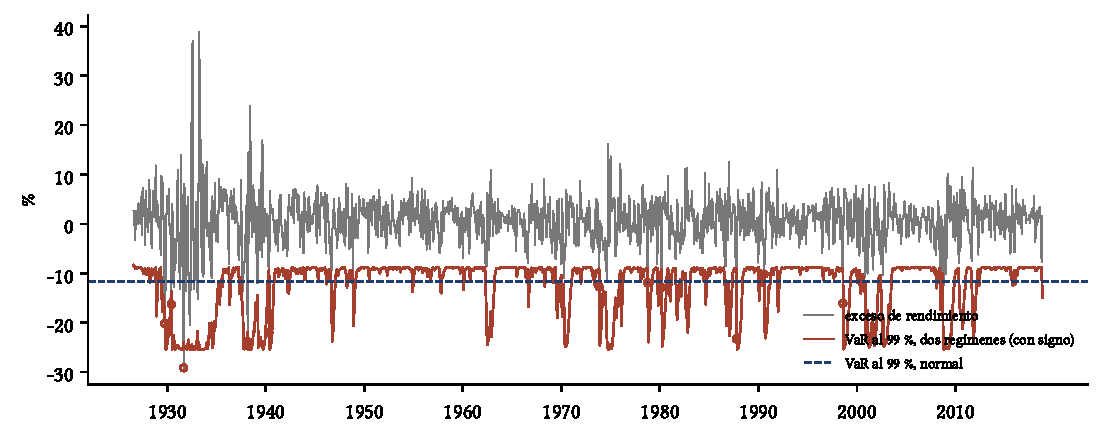
\includegraphics[width=\linewidth]{graficos/cap17_ej05_var.pdf}
\caption{Exceso de rendimiento mensual con el VaR al 99\,\% del modelo de dos regímenes (rojo, con sus excepciones marcadas) y
el de la normal (azul discontinua).}
\label{fig:var17}
\end{figure}

\begin{conclusion}
Un modelo de regímenes produce un VaR que se adapta a las crisis y supera las pruebas de cobertura e independencia donde el
modelo constante falla. Es una alternativa al GARCH con una interpretación directa: la probabilidad de estar en crisis.
\end{conclusion}
\end{ejresuelto}

% ---------------------------------------------------------------------
\section{Ejercicios propuestos}
% ---------------------------------------------------------------------

\begin{enumerate}[label=\textbf{\thechapter.\arabic*},leftmargin=*,itemsep=6pt]
  \item Con $p_{11}=0{,}95$ y $p_{22}=0{,}80$, calcule $\pi_1$, las duraciones esperadas y $\lambda$. \textit{Respuesta: $\pi_1=0{,}8$;
  20 y 5 períodos; $\lambda=0{,}75$.}

  \item Con $\boldsymbol\pi=(0{,}8;\,0{,}2)$, $\boldsymbol\mu=(1;\,-2)$ y $\boldsymbol\sigma=(4;\,10)$, calcule la media y la desviación estándar de
  la mezcla. \textit{Respuesta: $0{,}4$ y $\sqrt{34{,}24}=5{,}852$.}

  \item Con los parámetros del ejercicio anterior, $p_{11}=0{,}95$, $p_{22}=0{,}80$, $\boldsymbol\xi_{t-1\mid t-1}=(0{,}9;\,0{,}1)$ e
  $y_t=-8$, aplique un paso del filtro de Hamilton. \textit{Respuesta: $\boldsymbol\xi_{t\mid t-1}=(0{,}875;\,0{,}125)$;
  $\eta=(0{,}00793;\,0{,}03332)$; $\boldsymbol\xi_{t\mid t}=(0{,}625;\,0{,}375)$.}

  \item Demuestre que, si $\mu_1\neq\mu_2$ pero $\sigma_1=\sigma_2$, la mezcla también tiene autocorrelación en niveles:
  $\Cov(y_t,y_{t-k})=(\mu_1-\mu_2)^2\pi_1\pi_2\lambda^k$.

  \item Demuestre que la log-verosimilitud no disminuye en una iteración del EM. (Sugerencia: use la desigualdad de Jensen
  sobre $\ln f(\mathcal Y_T)=\ln\sum_{s}f(\mathcal Y_T,s)$.)

  \item \emph{(Simulación.)} Simule 200 muestras de 1\,109 meses de una normal con la media y la varianza del mercado, estime
  en cada una el modelo de dos regímenes y calcule $LR=2(\ell_2-\ell_1)$. Compare el percentil 95 del $LR$ simulado con el de
  una $\chi^2_4$. ¿Por qué difieren?

  \item \emph{(Con datos del BCRP.)} Estime el modelo B del Ejercicio~\ref{ej:produccion} con la variación anual del PBI mensual
  del Perú. ¿Identifica el régimen de recesión 1998--1999, 2009 y 2020?

  \item \emph{(Con datos.)} Repita el Ejercicio~\ref{ej:var17} reestimando el modelo cada 12 meses con los datos disponibles hasta
  esa fecha, desde 1950. ¿Siguen pasando las pruebas?
\end{enumerate}

% ---------------------------------------------------------------------
\section{Resumen de fórmulas}
% ---------------------------------------------------------------------

\begin{table}[H]
\centering\small
\begin{tabular}{@{}ll@{}}
\toprule
Concepto & Fórmula \\
\midrule
Estacionaria y duración & $\pi_1=\frac{1-p_{22}}{2-p_{11}-p_{22}}$;\quad $\E[D_i]=\frac1{1-p_{ii}}$;\quad $\lambda=p_{11}+p_{22}-1$ \\
Momentos de la mezcla & $\Var(y)=\sum_j\pi_j\sigma_j^2+\sum_j\pi_j(\mu_j-\bar\mu)^2$ \\
Agrupamiento & $\Cov(y_t^2,y_{t-k}^2)=(\sigma_1^2-\sigma_2^2)^2\pi_1\pi_2\lambda^k$ \\
Filtro de Hamilton & $\xi_{j,t\mid t}=\xi_{j,t\mid t-1}\eta_{jt}/\sum_k\xi_{k,t\mid t-1}\eta_{kt}$;\quad $\boldsymbol\xi_{t+1\mid t}=P'\boldsymbol\xi_{t\mid t}$ \\
Verosimilitud & $\ell=\sum_t\ln\sum_j\xi_{j,t\mid t-1}\eta_{jt}$ \\
Suavizador de Kim & $\xi_{i,t\mid T}=\xi_{i,t\mid t}\sum_jp_{ij}\,\xi_{j,t+1\mid T}/\xi_{j,t+1\mid t}$ \\
Paso M & $\hat\mu_j=\frac{\sum_t\hat\xi_{jt}y_t}{\sum_t\hat\xi_{jt}}$;\quad $\hat\sigma_j^2=\frac{\sum_t\hat\xi_{jt}(y_t-\hat\mu_j)^2}{\sum_t\hat\xi_{jt}}$;\quad $\hat p_{ij}=\frac{\hat n_{ij}}{\sum_k\hat n_{ik}}$ \\
\bottomrule
\end{tabular}
\caption{Fórmulas principales del Capítulo 17.}
\end{table}

\section*{Referencias}
\begin{itemize}[leftmargin=*]
  \item Ang, A. y Timmermann, A. (2012). Regime changes and financial markets. \emph{Annual Review of Financial Economics}, 4,
        313--337.
  \item Dempster, A. P., Laird, N. M. y Rubin, D. B. (1977). Maximum likelihood from incomplete data via the EM algorithm.
        \emph{Journal of the Royal Statistical Society, Series B}, 39(1), 1--38.
  \item Garcia, R. (1998). Asymptotic null distribution of the likelihood ratio test in Markov switching models.
        \emph{International Economic Review}, 39(3), 763--788.
  \item Hamilton, J. D. (1989). A new approach to the economic analysis of nonstationary time series and the business cycle.
        \emph{Econometrica}, 57(2), 357--384.
  \item Hamilton, J. D. (1990). Analysis of time series subject to changes in regime. \emph{Journal of Econometrics}, 45(1--2),
        39--70.
  \item Hamilton, J. D. (1994). \emph{Time Series Analysis}, cap. 22. Princeton University Press.
  \item Hansen, B. E. (1992). The likelihood ratio test under nonstandard conditions: Testing the Markov switching model of GNP.
        \emph{Journal of Applied Econometrics}, 7(S1), S61--S82.
  \item Kim, C.-J. (1994). Dynamic linear models with Markov-switching. \emph{Journal of Econometrics}, 60(1--2), 1--22.
  \item Kim, C.-J. y Nelson, C. R. (1999). \emph{State-Space Models with Regime Switching}. MIT Press.
  \item Krolzig, H.-M. (1997). \emph{Markov-Switching Vector Autoregressions}. Springer.
\end{itemize}
